\section{EL SISTEMA DODECAFÓNICO DE SCHOENBERG}\label{ch:dodecafonismo}
	\subsection{Los postulados del dodecafonismo}
		El dodecafonismo es un sistema compositivo que predetermina la melodía y la armonía a partir de una ordenación de las doce notas de la escala cromática, que se llama \textit{serie}. Ésta y algunas de sus transformaciones son los ladrillos con los que se construyen las alturas de las notas; son el único material que se puede utilizar. 
		
		El resto de elementos de la pieza, como el número de instrumentos, el ritmo, el carácter, la textura o las dinámicas, se dejan a discreción del compositor. No serializar todos los {conjuntos} será la principal crítica al dodecafonismo por parte de los compositores serialistas que sucedieron a su creador, Arnold Schoenberg. Para los serialistas integrales, como Pierre Boulez, aquello restaba cohesión al modelo compositivo; para los dodecafonistas, aportaba libertad. 
		%
		\cite{boulez}
		
		Precisamente la predeterminación dodecafónica, aunque parece limitante, permite realizaciones musicales y estilos de composición muy diferentes: Schoenberg daba un tratamiento tradicional a sus obras, ya que aún admiraba las formas clásicas; Alban Berg iba más allá al utilizar series que recordaban a las tríadas tonales; y, en cambio, Anton Webern evitaba radicalmente cualquier asociación con la tradición. 
		
		Schoenberg definió su sistema musical a partir de cuatro postulados que, en realidad, se basan en principios matemáticos \cite{dominguez}:
		
		\emph{1. La serie \emph{[sobre la que se construye la obra dodecafónica]} consta de las doce notas de la escala cromática dispuestas en un orden lineal específico.}
		
		\emph{2. Ninguna nota aparece más de una vez en la serie.}
		
		Los dos primeros postulados expresan que una obra dodecafónica fundamenta su estructura sobre una {permutación} de la escala de doce semitonos. Dicha permutación $\sigma$ es una biyección del conjunto numerado de las doce notas \{Do = 0, Do\# = 1, Re = 2, Re\# = 3, Mi = 4, Fa = 5, F\# = 6, Sol = 7, Sol\# = 8, La = 9, La\# = 10, Si = 11\} consigo mismo, y se representa de esta forma:
		
		\[
			\drow{
				\sigma(0),\sigma(1),\sigma(2),\sigma(3),\sigma(4),\sigma(5),\sigma(6),\sigma(7),\sigma(8),\sigma(9),\sigma(10),\sigma(11)
			}
		\]
		
		La permutación $\sigma(m)$, con $m\in \mathbb{Z} / (12)$%{\footnotemark}
		, pertenece al grupo simétrico de orden 12: $\sigma\in$ S$_{12}$. Por ejemplo, en la Suite para piano Op. 25 Schoenberg utiliza como serie original en todos los movimientos de la obra la siguiente permutación $\sigma$:
		
		\[\sigma=\drow{4,5,7,1,6,3,8,2,11,0,9,10}\]	
		\begin{center}
			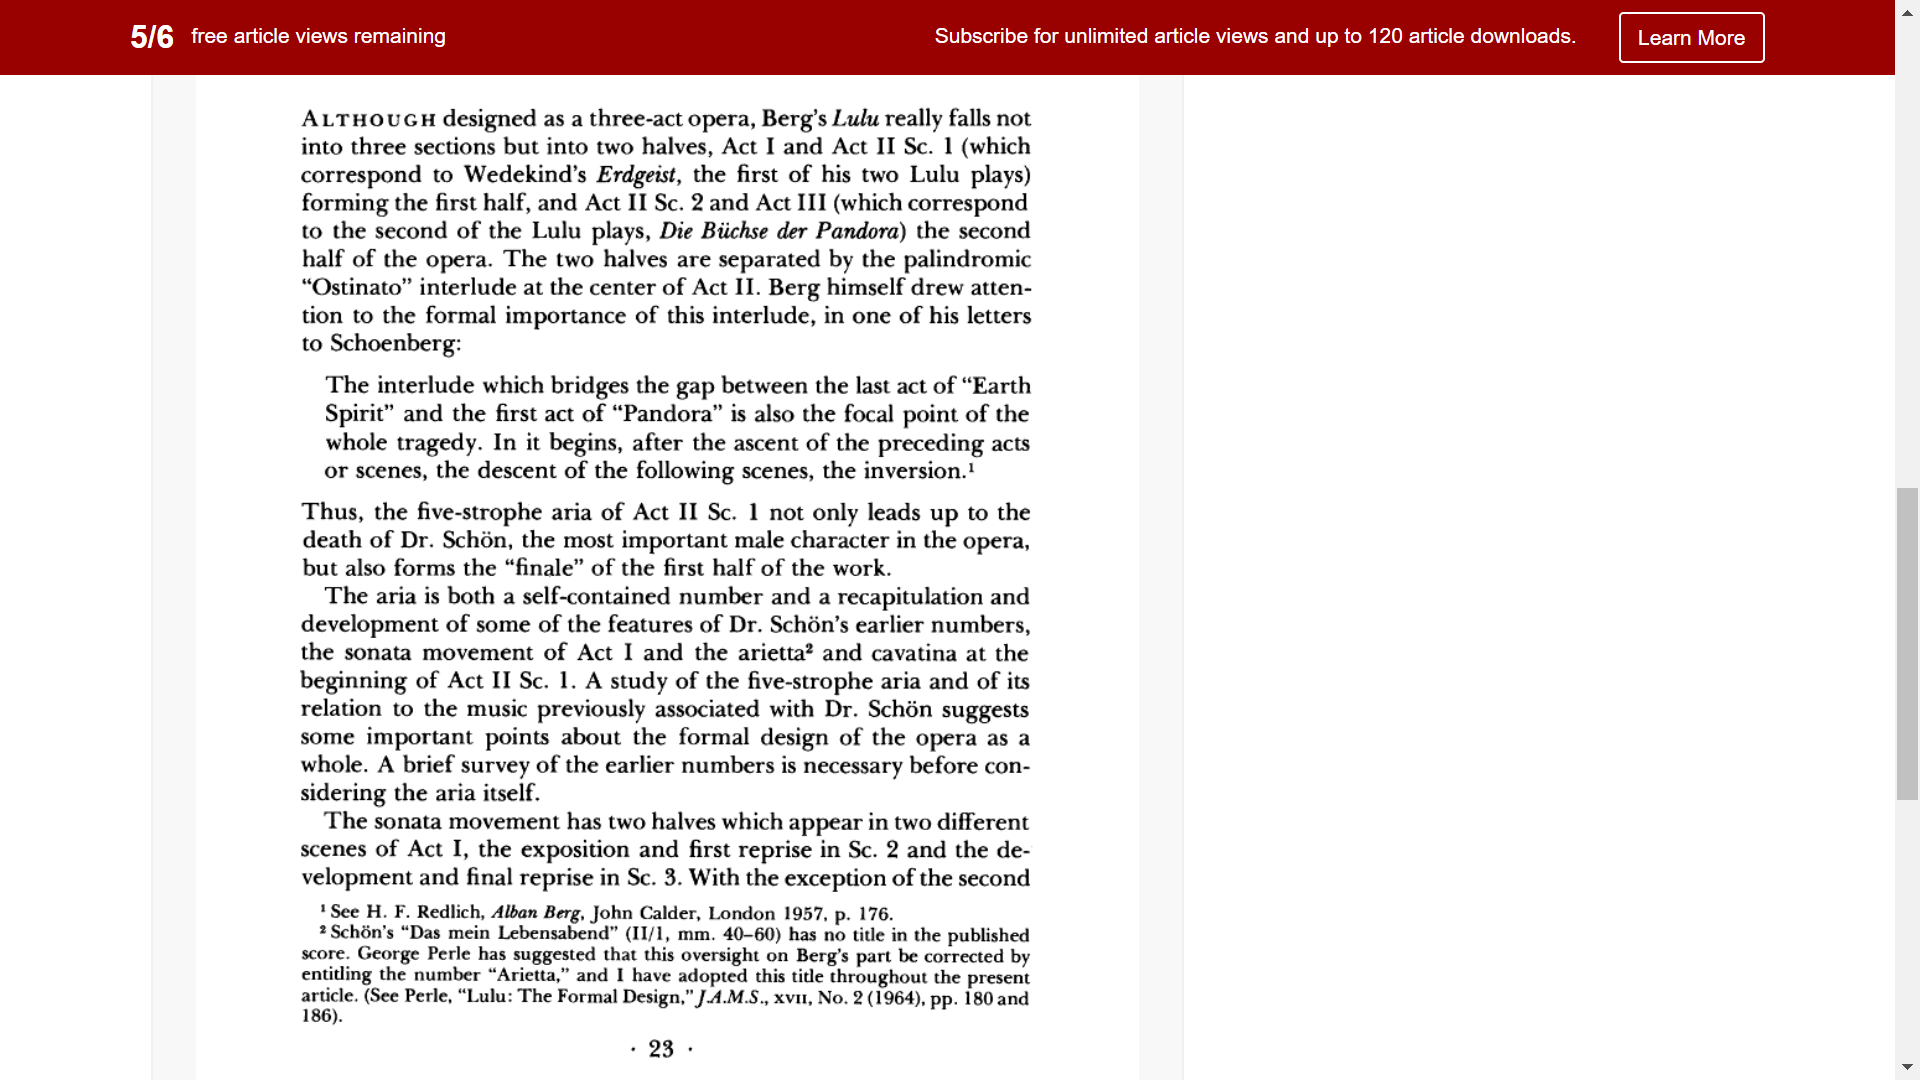
\includegraphics[width=12.1cm]{1.png}
		\end{center}
		
		\emph{3. La serie será expuesta en cualquiera de sus aspectos lineales: original, inversión, retrogradación de la original y retrogradación de la inversión.}
		 
		\emph{4. La serie puede usarse en sus cuatro aspectos desde cualquier nota de la escala.}
		
		Los dos últimos postulados amplían los recursos compositivos al admitir la transformación de la serie original mediante \emph{inversión}, \emph{retrogradación}, \emph{inversión retrógrada} y \emph{transposición}. %({No confundir con un 2-ciclo. Una transposición musical se corresponde con una traslación matemática.}) 
		El compositor puede utilizar cualquiera de las transformaciones de una serie al componer su obra dodecafónica. El conjunto de series que puede utilizar, que viene dado por la serie original y todas sus posibles transformaciones, se conoce como \emph{espectro serial}.
		%
		\cite{dominguez}
		
	\subsection{Las transformaciones de una serie}
		\label{transPsi}
		Transformar una serie es matemáticamente equivalente a aplicar una {función} sobre la serie, y que asocie esa permutación a la permutación transformada. Por tanto, cualquier función transformativa $\Psi$ se aplica sobre el conjunto de las permutaciones, {S$_{12}$}.
		
	\subsubsection{Transposiciones}
		La \emph{transposición}, mencionada en el cuarto postulado, consiste en subir o bajar la serie original un número determinado de semitonos. Por tanto, no se modifican los intervalos entre las notas, sino solamente la altura a la que está la serie. Ya que consideraremos todas las octavas equivalentes, debemos trabajar {módulo} 12.
		
		La serie transportada k semitonos (con k constante), $\mbox{T}^{{\mbox{k}}}(\sigma)$, se construye sumando k a $\sigma$ (mod. 12):
		\[\mbox{T}^{{\mbox{k}}}(\sigma(m))=\sigma(m)+{\mbox{k}}\]		
		{\[
		\mbox{T}^{{\mbox{k}}}=
		\left(\begin{array}{*{7}c}
			0&1&2&&9&10&11\\
			\sigma(0)+{\mbox{k}}&\sigma(1)+{\mbox{k}}&\sigma(2)+{\mbox{k}}&
			\cdots&
			\sigma(9)+{\mbox{k}}&\sigma(10)+{\mbox{k}}&\sigma(11)+{\mbox{k}}\\
		\end{array}\right)
		\]}
		
		A su vez, T$^{\mbox{k}}$ se forma al componer k transposiciones de 1 semitono: $\mbox{T}^{\mbox{k}}=\mbox{T}^1\circ\mbox{T}^1\circ\ldots\circ\mbox{T}^1$, k veces. Debido a que k es en realidad el exponente en la potencia de T, se coloca este número como superíndice.
		
		Históricamente, la notación $\Psi_{\mbox{k}}$, $\Psi^{\mbox{k}}$ o $\Psi({\mbox{k}})$ se ha usado en sustitución de la composición de la transposición T$^{\mbox{k}}$ y otra función $\Psi$, en el respectivo orden: $\Psi^{\mbox{k}}=\Psi \circ \mbox{T}^{\mbox{k}} = \Psi(\mbox{T}^{\mbox{k}})$. Sin embargo, esta notación es especialmente ambigua y confusa, sobre todo al trabajar con funciones no conmutativas -- cuando importa el orden en el que estén T y $\Psi$. Por ello, es preferible ceñirse a la notación estrictamente matemática; es decir, a la composición de funciones, aun omitiendo el símbolo $\circ$: \cancel{$\Psi_{\mbox{k}}$}, \cancel{$\Psi^{\mbox{k}}$}, \cancel{$\Psi({\mbox{k}})$} $\rightarrow \Psi\mbox{T}^{\mbox{k}}$
		
		Una posible serie transportada sobre la permutación $\sigma$ de la Suite para piano Op. 25, con k $= 6$, es la siguiente serie T$^6$:
		\[\mbox{T}^6=\drow{10,11,1,7,0,9,2,8,5,6,3,4}\]	
		\begin{center}
			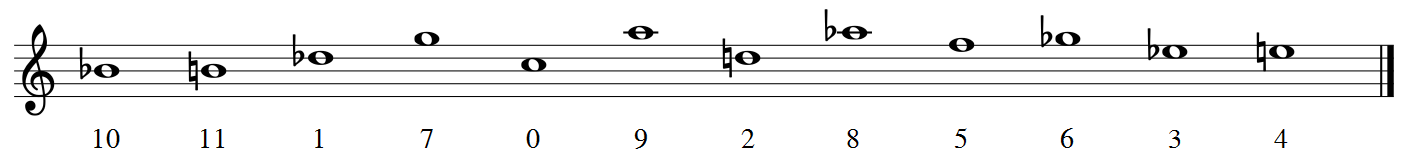
\includegraphics[width=12.1cm]{2.png}
		\end{center}
		
	\subsubsection{Retrogradación}
		La \emph{retrogradación} consiste en leer la serie original desde la nota final hacia atrás, es decir, aplicar a la serie una simetría especular. De este modo, la primera nota irá al último puesto, la segunda al penúltimo, y así sucesivamente.
		
		La serie retrógrada se construye de esta forma:
		\[\mbox{R}(\sigma(m))=\sigma(-1-m)\]
		\[{\mbox{R}=\drow{\sigma(11),\sigma(10),\sigma(9),\sigma(8),\sigma(7),\sigma(6),\sigma(5),\sigma(4),\sigma(3),\sigma(2),\sigma(1),\sigma(0)}}\]
			
		La serie retrógrada sobre la permutación $\sigma$ de la Suite Op. 25 es la siguiente serie R:	
		\[\mbox{R}=\drow{10,9,0,11,2,8,3,6,1,7,5,4}\]		
		\begin{center}
			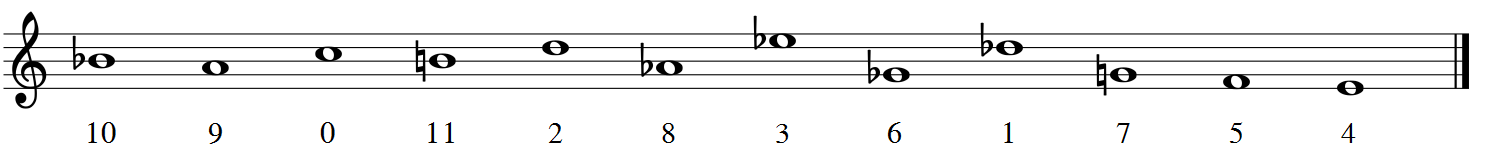
\includegraphics[width=12.1cm]{3.png}
		\end{center}
		
	\subsubsection{Inversión}
		La \emph{inversión} consiste en cambiar la dirección --de ascendente a descendente, y viceversa-- de los intervalos entre cada nota de la serie. Si el primer intervalo en la serie original $\sigma$ es de $+k$, el primer intervalo en la serie invertida I será de $-k$ (mod. 12), por lo que debemos cambiar el signo de $\sigma$ para construir I. Además, queremos que la primera nota de ambas series, I($\sigma$(0)) y $\sigma$(0), coincidan, así que debemos transportar la serie ($-\sigma$) un número $\lambda$ de semitonos para que esta condición se cumpla:
		\begin{align*}
		\mbox{I}(\sigma(0))=-\sigma(0)+\lambda&=\sigma(0)\\
		\implies \lambda&=2\sigma(0)
		\end{align*}
		Por tanto, la serie invertida se construye de esta forma:
		\[\mbox{I}(\sigma(m))=-\sigma(m)+2\sigma(0)\]
		
		\[\mbox{I}=\left(\begin{matrix}0&1&2&&10&11\\\sigma(0)&-\sigma(1)+2\sigma(0)&-\sigma(2)+2\sigma(0)&\ldots&-\sigma(10)+2\sigma(0)&-\sigma(11)+2\sigma(0)\\\end{matrix}\right)\]
		
		La serie invertida sobre la permutación $\sigma$ de la Suite Op. 25 es la siguiente serie I:
		\[\mbox{I}=\drow{4,3,1,7,2,5,0,6,9,8,11,10}\]		
		\begin{center}
			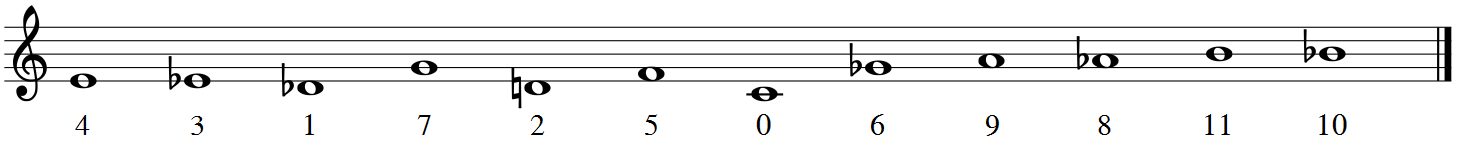
\includegraphics[width=12.1cm]{4.png}
		\end{center}
				
		En total, obtendremos 48 series -- aunque no obligatoriamente distintas entre sí -- pertenecientes a un solo espectro serial. Hay 12 series originales sobre cada una de las doce notas, 12 series retrógradas, 12 invertidas y 12 series sobre las que se aplica tanto la retrogradación como la inversión. A continuación se muestra la sintaxis simple junto a la matemática:
		
		\begin{multicols}{2}
			\underline{Sintaxis simple}
			
			T$_0$, T$_1$, T$_2$\ldots
			
			R$_0$, R$_1$, R$_2$\ldots
			
			I$_0$, I$_1$, I$_2$\ldots
			
			IR$_0$, IR$_1$, IR$_2$\ldots
			
			\underline{Sintaxis matemática}
			
			T$^0$, T$^1$, T$^2$\ldots
			
			R, RT$^1$, RT$^2$\ldots
			
			I, IT$^1$, IT$^2$\ldots
			
			IR, IRT$^1$, IRT$^2$\ldots
		\end{multicols}
	
	\subsection{Matrices dodecafónicas}
		
		Dada una serie, su matriz dodecafónica es una representación visual de su espectro serial; es decir, del conjunto de series derivadas de esa serie. El espectro serial es todo el material compositivo sonoro del que se dispone para la composición de una obra dodecafónica. Al poder ordenar y disponer la información en una tabla, el compositor puede acceder a toda ella al mismo tiempo sin tener que calcular cada serie individualmente.		
		
		La matriz se lee en la dirección en la que aparece el nombre de la serie. Las series T se leen de izquierda a derecha, mientras que las series R de derecha a izquierda. Las series I se leen de arriba a abajo y las IR/RI de abajo a arriba.
		
		He creado un programa que devuelve en formato \LaTeX{} la matriz correspondiente a cualquier serie dodecafónica que se introduzca en teclado, además de producir la nomenclatura simple para cada serie. El código, escrito en C++, se puede encontrar en el enlace \url{https://gitlab.com/dodecafonismo/cppmatrices}.
		
		A continuación, se incluye la matriz dodecafónica de la serie P de la Suite Op. 25 de Schoenberg. Mientras que la mayoría de tablas tienen dos filas inferiores, que se corresponden con las distintas nomenclaturas de RI e IR para una misma serie -- ya que normalmente no conmutan --, en la matriz de la serie P sí coinciden.
		
		\[\begin{array}{l|cccccccccccc|r}
		&\mbox{I}_{0}&\mbox{I}_{1}&\mbox{I}_{3}&\mbox{I}_{9}&\mbox{I}_{2}&\mbox{I}_{11}&\mbox{I}_{4}&\mbox{I}_{10}&\mbox{I}_{7}&\mbox{I}_{8}&\mbox{I}_{5}&\mbox{I}_{6}&\\
		\hline
		\mbox{T}_{0}&4&5&7&1&6&3&8&2&11&0&9&10&\mbox{R}_{0}\\
		\mbox{T}_{11}&3&4&6&0&5&2&7&1&10&11&8&9&\mbox{R}_{11}\\
		\mbox{T}_{9}&1&2&4&10&3&0&5&11&8&9&6&7&\mbox{R}_{9}\\
		\mbox{T}_{3}&7&8&10&4&9&6&11&5&2&3&0&1&\mbox{R}_{3}\\
		\mbox{T}_{10}&2&3&5&11&4&1&6&0&9&10&7&8&\mbox{R}_{10}\\
		\mbox{T}_{1}&5&6&8&2&7&4&9&3&0&1&10&11&\mbox{R}_{1}\\
		\mbox{T}_{8}&0&1&3&9&2&11&4&10&7&8&5&6&\mbox{R}_{8}\\
		\mbox{T}_{2}&6&7&9&3&8&5&10&4&1&2&11&0&\mbox{R}_{2}\\
		\mbox{T}_{5}&9&10&0&6&11&8&1&7&4&5&2&3&\mbox{R}_{5}\\
		\mbox{T}_{4}&8&9&11&5&10&7&0&6&3&4&1&2&\mbox{R}_{4}\\
		\mbox{T}_{7}&11&0&2&8&1&10&3&9&6&7&4&5&\mbox{R}_{7}\\
		\mbox{T}_{6}&10&11&1&7&0&9&2&8&5&6&3&4&\mbox{R}_{6}\\
		\hline
		&\mbox{IR}_{0}&\mbox{IR}_{1}&\mbox{IR}_{3}&\mbox{IR}_{9}&\mbox{IR}_{2}&\mbox{IR}_{11}&\mbox{IR}_{4}&\mbox{IR}_{10}&\mbox{IR}_{7}&\mbox{IR}_{8}&\mbox{IR}_{5}&\mbox{IR}_{6}&\\
		\hline
		&\mbox{RI}_{0}&\mbox{RI}_{1}&\mbox{RI}_{3}&\mbox{RI}_{9}&\mbox{RI}_{2}&\mbox{RI}_{11}&\mbox{RI}_{4}&\mbox{RI}_{10}&\mbox{RI}_{7}&\mbox{RI}_{8}&\mbox{RI}_{5}&\mbox{RI}_{6}&
		\end{array}\]
	
		Por otro lado, he escrito otro programa en el propio lenguaje \LaTeX{} que crea esta misma tabla con el comando \verb|\dmatrix|, y tiene cualquier serie como argumento: \verb|\dmatrix{4,5,7,1,6,3,8,2,11,0,9,10}|. %El código se encuentra en el Anexo \ref{app:latex}, página \pageref{app:latex1}. 
		El código se encuentra en mi paquete de \LaTeX{} \texttt{ddphonism}, incluido en el enlace  \url{https://www.ctan.org/pkg/ddphonism}.
		La tabla aparece sin el orlado de nomenclaturas:
		
		\dmatrix{4,5,7,1,6,3,8,2,11,0,9,10}
		
		También he creado una página interactiva que genera matrices de cualquier serie para cualquier longitud serial, además de generar series aleatorias. Permite escoger entre dos numeraciones y dos nomenclaturas. Está escrita en Elm y el código puede encontrarse en \url{https://gitlab.com/dodecafonismo/matrices}.
		
%			\qrcode{https://matrices.netlify.com/}
			
			En este enlace se encuentra la aplicación web. Sus instrucciones de uso se encuentran al final de la página: \url{https://matrices.netlify.com/}.